In this appendix, we supplement the following materials to support the findings and conclusions drawn in the main body of this paper.

\startcontents[appendices]
\printcontents[appendices]{l}{1}{\setcounter{tocdepth}{3}}


\clearpage


\section{Training and metric details}
\label{sec:training_and_metrics_details}

\subsection{Training configuration}

The training of OccSim's two components—W-DiT and the Layout Generator—was conducted separately as follows. For W-DiT, we trained for 200 epochs on 4 Blackwell RTX Pro 6000 GPUs with a batch size of 32. Training on the Nuscenes dataset took approximately 100 GPU hours. For the Layout Generator, we trained for 500 epochs on 8 A100 80G GPUs, taking approximately 160 GPU hours. All of the experiments used AdamW with cosine annealing, decaying the learning rate from 3.2e-5 to 3.2e-6. 

In Eq. \ref{eq:total_loss}, we set $\lambda=2$, with 20\% possiblilty to drop condition during training for classifier free guidance \cite{ho2022classifier} in sampling stage. When generating $\mathbf{M}_{\text{rand}}$, we control the maximum of overall masked region $\mathbf{M}_{\text{mask}}$ between 10\% to 50\% of the full latent size. $\epsilon$ in Eq. \ref{eq:total_loss} is sampled from $\text{sigmoid}(\mathcal{N}(0, I))$. 


\subsection{Augmentation in Layout generator}
\label{sec:appendix_augmentations}


Theoretically, the distribution of valid vehicle behaviors given a specific map representation, denoted $P(\mathcal{H} | \mathbf{z}_{t})$, is inherently highly multimodal, as various driving intentions can perfectly align with the same static environment. However, direct optimization on a finite training dataset $\mathcal{D} = \{(\mathbf{z}_{t}^{(i)}, \mathcal{H}^{(i)})\}_{i=1}^{N}$ poses a severe risk of overfitting, as the number of samples is only 28K to train the DiT-S. In practice, for any specific scene $\mathbf{z}_{t}^{(i)}$ in the log, we only observe a single deterministic realization of the vehicles' behavior $\mathcal{H}^{(i)}$. Consequently, without proper regularization, model tend to memorize these exact map-action pairs, effectively collapsing the learned conditional distribution into a Dirac delta function, $P_{\theta}(\mathcal{H} | \mathbf{z}_{t}^{(i)}) \approx \delta(\mathcal{H} - \mathcal{H}^{(i)})$. 

To prevent the model from memorizing spurious correlations between specific voxel arrangements and deterministic position, we introduce the data augmentation in layout generator training. By applying paired spatial transformations $\mathcal{T}$ to both the condition and the target, i.e., $(\mathcal{T}(\mathbf{z}_{t}), \mathcal{T}(\mathcal{H}))$, we artificially expand the support of the empirical distribution. Specifically, we introduce a two-stage data augmentation pipeline comprising agent-level perturbations and global spatial transformations. 

First, to manage scene density and prevent the model from overfitting to overly crowded environments, we cap the maximum number of vehicles per frame at 10; if a frame contains $N > 10$ vehicles, we uniformly sample a subset of exactly $10$ vehicles without replacement, ensuring each vehicle has an equal retention probability of $10/N$. For each retained vehicle, we project it onto a 2D spatial heatmap $\mathcal{H} \in \mathbb{R}^{200 \times 200 \times 1}$ as a Gaussian distribution. Specifically, the Gaussian is centered at the vehicle's spatial coordinates with a kernel radius of 3. To simulate positional uncertainty and enrich the local behavioral manifold, we independently perturb the center of each Gaussian, randomly shifting it within a local $5 \times 5$ neighborhood restricted to the drivable surface area. 

Following this localized perturbation, we apply rigid global transformations to the entire augmented scene (including both the occupancy map and the constructed heatmap $\mathcal{H}$). We uniformly sample and apply discrete rotations $\mathcal{R} \in \{90^\circ, 180^\circ, 270^\circ\}$ and axis-aligned reflections and axis-aligned reflections (flipping along the x- or y-axis). Crucially, identical spatial transformations are applied to the corresponding latent representations to maintain spatial alignment with $\mathcal{H}$. While such reflections fundamentally invert the handedness of the traffic rules (effectively synthesizing valid left-hand traffic scenarios from right-hand data), this joint transformation ensures that all local topological constraints and relative vehicle dynamics remain physically coherent. This composite strategy effectively artificially expands the empirical distribution, forcing the network to learn robust, viewpoint-invariant geometric representations.

\subsection{Additional metrics details}
\label{sec:appendix_training_details}

To evaluate the diversity of the generated stochastic rollouts, we employ two distinct metrics: Pairwise mIoU Diversity in the decoded semantic space, and the Vendi Score \cite{friedman2022vendi} in the latent feature space. 

For the decoded semantic space, we generate $N$ independent sequences over $\mathbb{T}$ frames using different random seeds. At any given timestep $t$, we compute the mean Intersection over Union ($\text{mIoU}$) across all semantic categories for every unique pair of generated occupancy grids. The Pairwise mIoU Diversity at time $t$ is then defined as the complement of the average pairwise similarity:
$$D_t = 1 - \frac{1}{|\mathcal{P}|}\sum_{(i,j)\in\mathcal{P}} \text{mIoU}_{t}^{(i,j)}$$
where $\mathcal{P} = \{(i,j) : 1 \le i < j \le N\}$ denotes the set of all unordered seed pairs. The rollout-level diversity is obtained by averaging $D_t$ over time.

To capture structural diversity in the latent space, we report the Vendi Score, which measures the effective sample size of the generated distributions. First, we extract frame-level features $\{x_i\}_{i=1}^N$ using pretrained encoders (i.e., the OccFM VAE encoder and the UniScenes AE encoder). We then compute a cosine similarity kernel matrix $\mathcal{Q}$, where its elements are given by $\mathcal{Q}_{ij} = (1 + \tilde{x}_i^\top \tilde{x}_j)/2$, with $\tilde{x}$ being the $\ell_2$-normalized feature. The Vendi Score is calculated as the exponential of the von Neumann entropy of the normalized kernel matrix $\hat{\mathcal{Q}} = \mathcal{Q}/\text{tr}(\mathcal{Q})$:
$$V = \exp \left( -\sum_\ell \lambda_\ell \log \lambda_\ell \right)$$
where $\{\lambda_\ell\}$ are the non-negative eigenvalues of $\hat{\mathcal{Q}}$.

Intuitively, the Vendi Score quantifies the effective number of distinct modes within a given set of generations. By evaluating the entropy of the similarity eigenspectrum, it properly penalizes highly correlated samples. A higher Vendi Score indicates that the generated occupancy features are widely distributed across the latent space, reflecting true structural and geometric diversity rather than minor variations of a single collapsed mode.

\section{Additional ablation experiments}

\subsection{Inference speed and condition comparison}

In the previous section, we demonstrated a comparison between our method and prior approaches in terms of realism. However, it is worth noting that our method also achieves significant improvements in real-time performance compared to them. In Tab. \ref{tab:efficiency_comparison}, we compares the time and FLOPS required for our method to generate a single frame.

\begin{table}[htbp]
    \centering
    \caption{Comparison of efficiency and computational cost among different methods. When evaluating the time taken by our method, we distribute the post-processing time evenly across each frame of the sequence generation. Each result was computed independently using an RTX4090. DOME and COME generate 6 frames together, ours is 1 single frame per step, for fair comparison, we keep measure the GFLOPS / inference time needed per single frame.}
    \label{tab:efficiency_comparison}
    \setlength{\tabcolsep}{6pt} % default is usually 6pt

    \begin{tabular}{lclrrr}
        \toprule
        Method & WM & Input & \#Params & $\frac{\text{Frames}}{\text{second}}$ & $\frac{\text{GFLOPS}}{\text{frame}}$ \\
        \midrule
        DOME & \ding{51} & 4 frames sem. occ.\&traj & 444.07M & 5.48 & 8891.98 \\
        COME & \ding{51} & 4 frames sem. occ.\&traj & 204.53M & 2.33 & 41333.17 \\
        InfiniCubes & \ding{53} & 1 frames sem. occ. & 831.75M & 0.02 & 990927.28 \\
        OccSim (Ours) & \ding{51} & 1 frames sem. occ. \& traj & 181.24M & 1.47 & 15570.18 \\
        \bottomrule
    \end{tabular}
\end{table}

\section{Additional visualization}

\subsection{Visualization of long-horizon rollouts}
From Fig. \ref{fig:w-dit_over_time}, we can clearly observe that our proposed W-DiT significantly extends the duration of stable rollout. Even after 3000 frames (1500s, approximately 25 minutes), the generated occupancy remains stable.
\begin{figure}[htb]
    \centering
    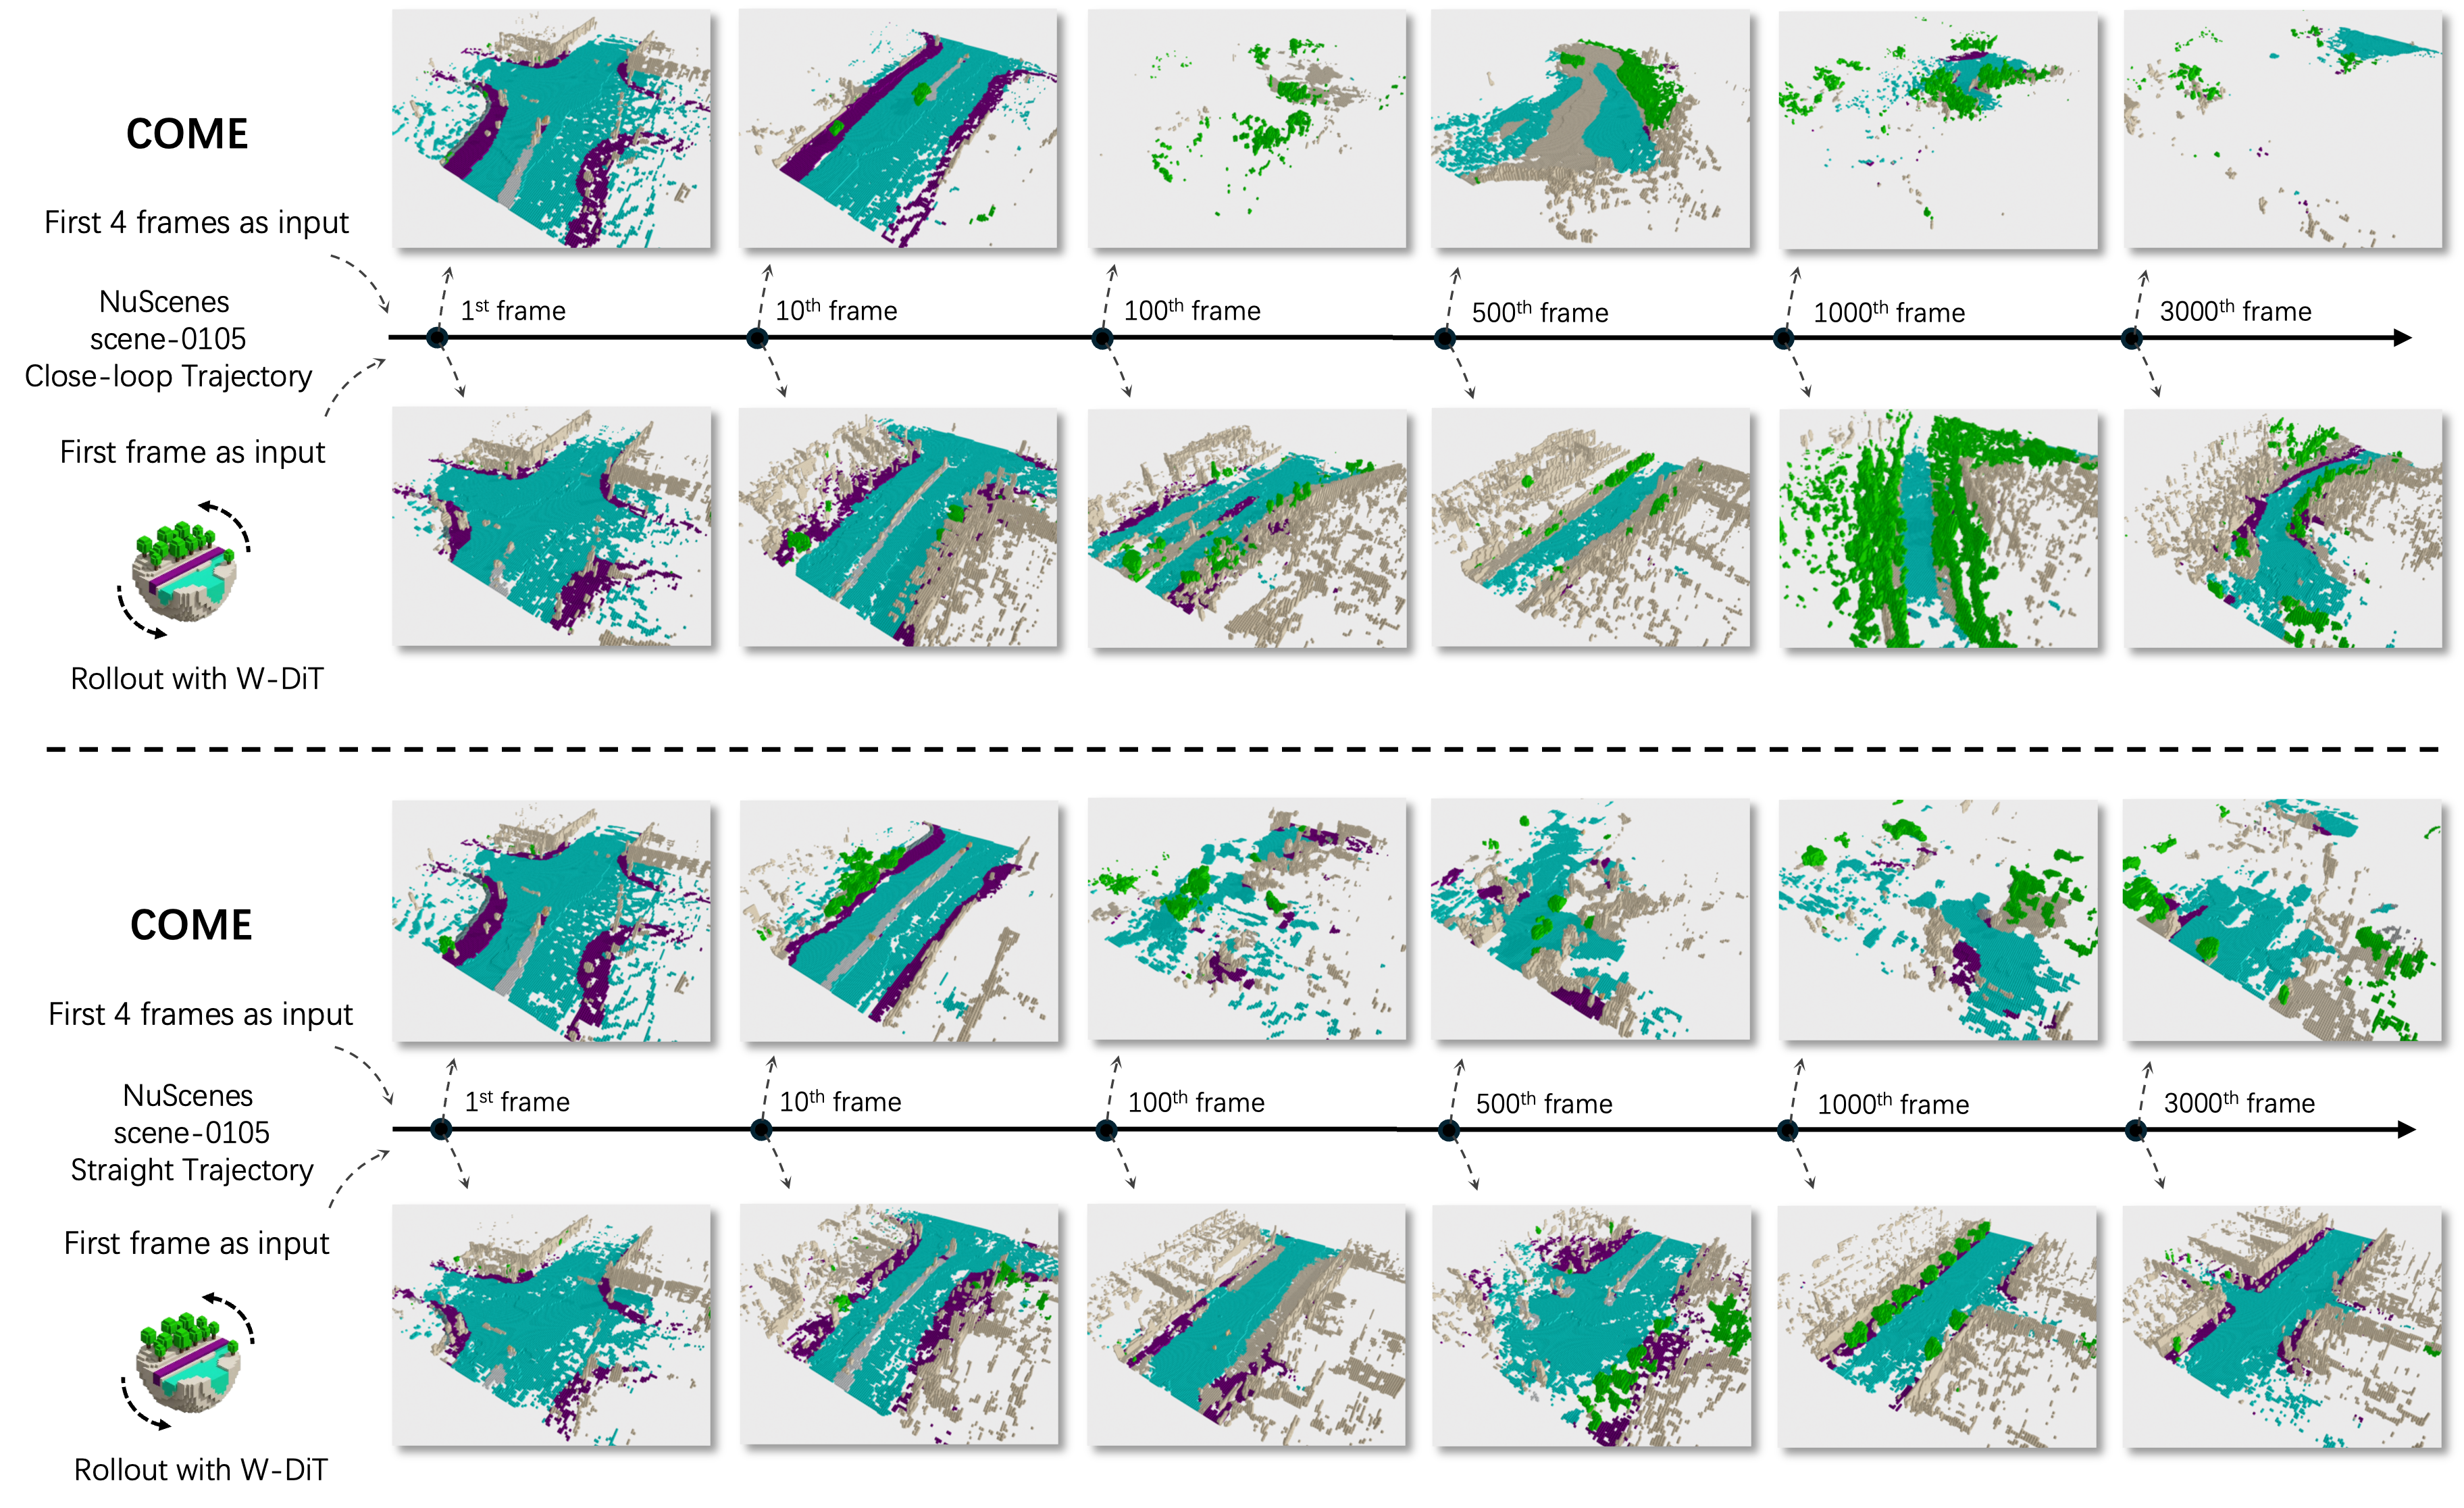
\includegraphics[width=\linewidth]{figures/time-index-compare.png}
    \caption{Qualitative comparison of two rollouts for two models: previous SOTA occupancy world model (first and third rows), and our model (second and fourth rows) at different horizons. Ours exhibits long-horizon stability under different trajectory input.}
    \label{fig:w-dit_over_time}
\end{figure}


\subsection{Visualization of trajectory shapes used in Fig.~\ref{fig:uncond_2d}}
\label{sec:appendix_trajectories}
To systematically evaluate the robustness of our model in long-horizon generation across diverse driving behaviors, we configure three distinct spatial trajectory profiles: Loop, Straight, and Turn. As illustrated in Fig. \ref{fig:traj_vis}, the trajectory generation process conditioned on is consist of  the initial ground-truth (GT) trajectory (highlighted in blue, encompassing frames 1–40) and extended trajectory with 3 modes (red lines). 
\begin{figure}[htb]
    \centering
    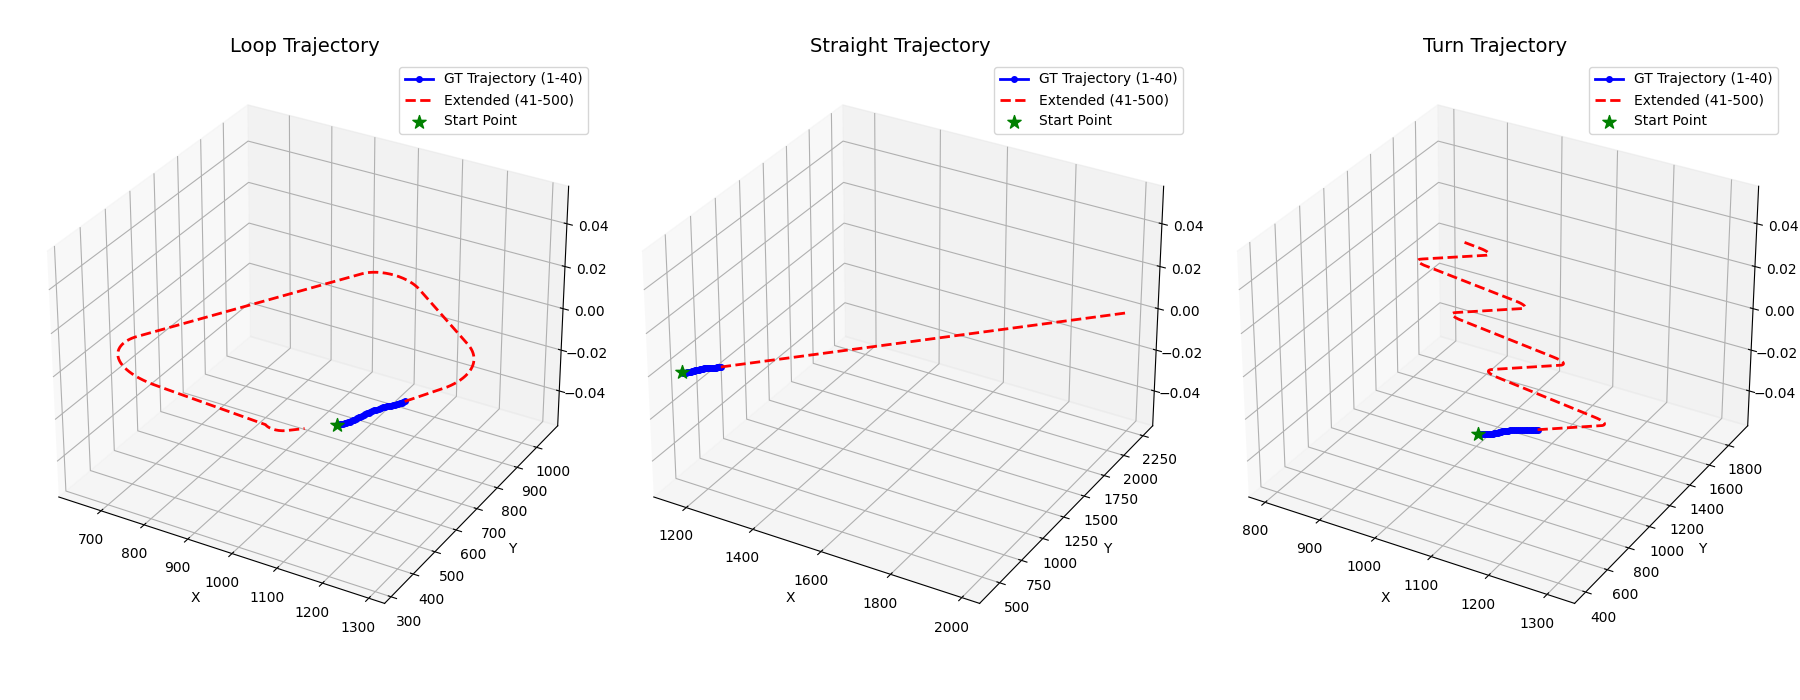
\includegraphics[width=0.85\linewidth]{figures/traj_3d.png}
    \caption{Visualization of trajectory shapes (Loop, Straight, and Turn) evaluated in Fig. 5. The green star indicates the starting point. The blue solid line denotes the initial ground-truth (GT) trajectory snippet (frames 1–40) used as the condition prompt, while the red dashed line represents the extended trajectory explicitly designed to guide the long-horizon generation. For visual clarity the displayed trajectories are truncated at 500 frames, whereas our actual synthesis spans up to 3000 frames.}
    \label{fig:traj_vis}
\end{figure}

\subsection{Visualization of chaos baseline constructed}
\label{sec:appendix_chaos}
As shown in Fig. \ref{fig:chaos}, the constructed ``chaos'' baseline primarily comprises severely fragmented road segments, topologically disconnected layouts, and large-scale empty regions. Consequently, as we mentioned in Fig. \ref{fig:uncond_2d}, any model yielding FID/KID scores above this baseline threshold can be deemed completely incapable of synthesizing large-scale, valid road networks. 

\begin{figure}[htbp]
    \centering
    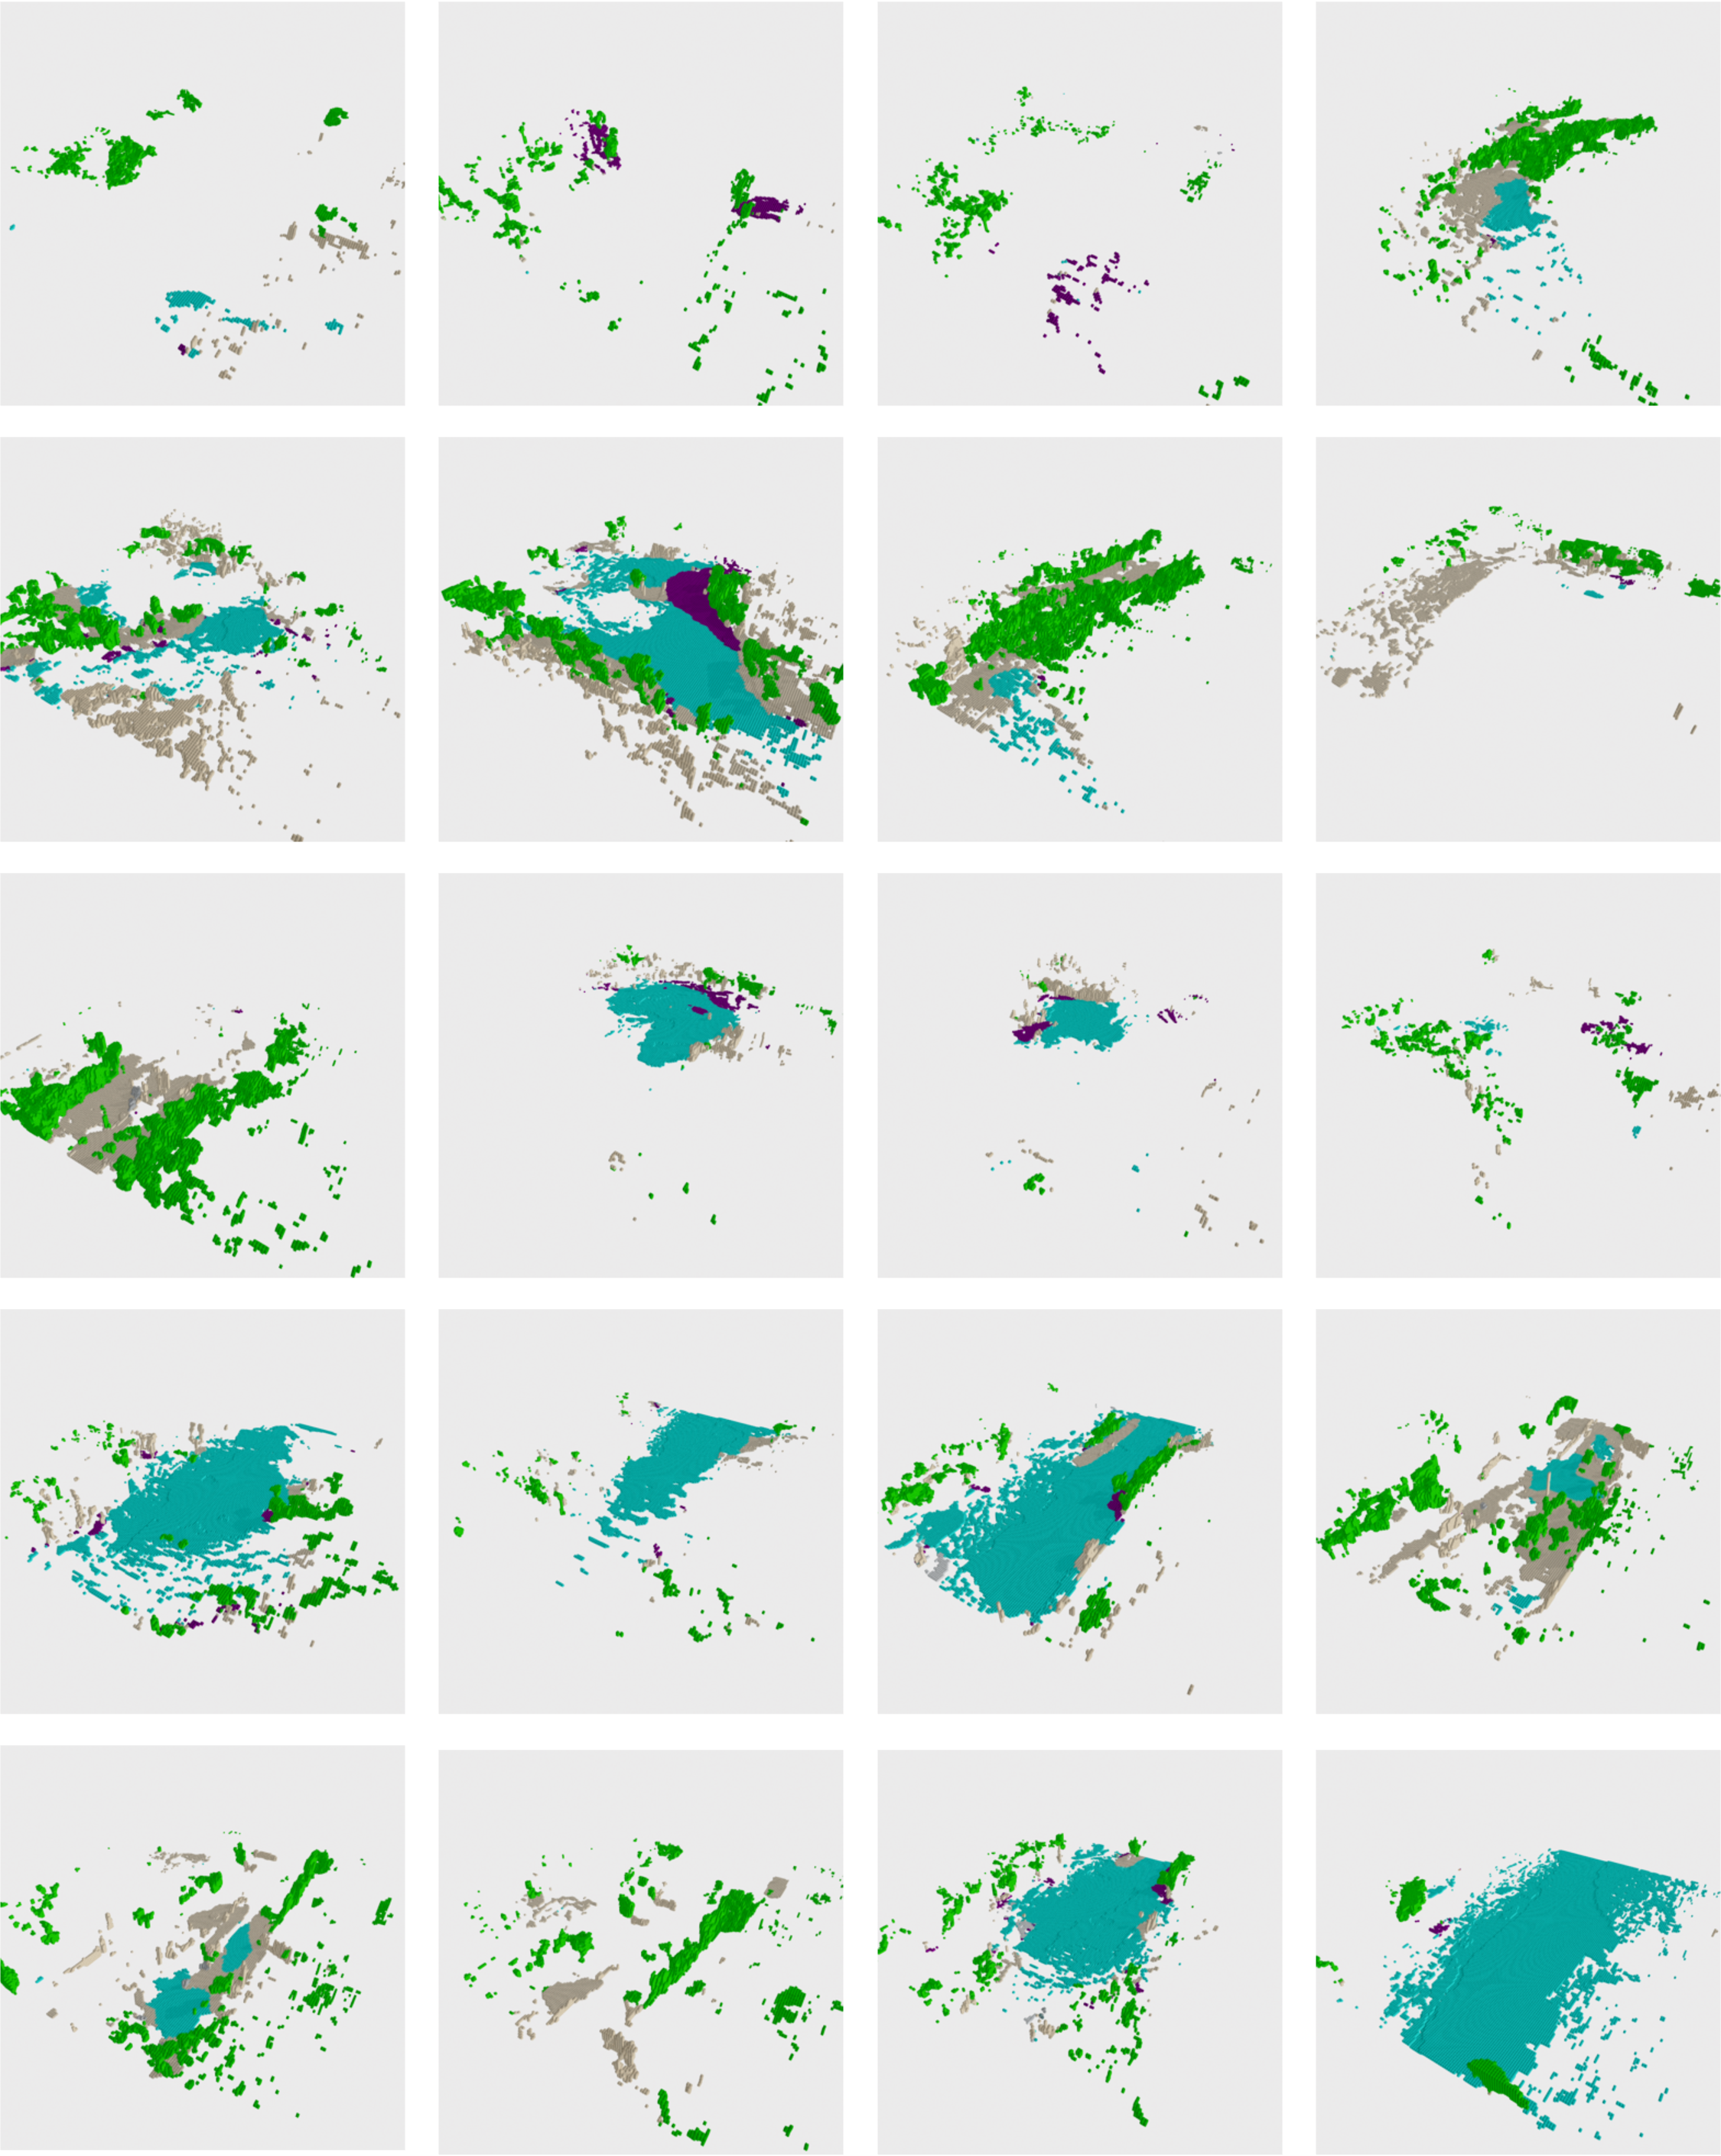
\includegraphics[width=\linewidth]{figures/chaos.png}
    \caption{Visualization of frames from the ``chaos'' baseline. We randomly visualize 20 frames from the 1000 samples pool. The semantic categories represented by colors here are consistent with those in Fig. \ref{fig:with_agent}. }
    \label{fig:chaos}
\end{figure}


\section{Algorithm details}
\label{sec:appendix_algorithms}

\subsection{Heuristic for Single frame fusion.} After we obtained the raw forecast observation $\{\mathcal{O}_i\}_{i}^{K}$ from the W-DiT based world model, we than use the following algorithm \ref{alg:keyframe_fusion} to fuse all frames to $\mathcal{M}_{\text{global}}$. 

\begin{algorithm}[h]
\caption{Two-pass Keyframe-based Occupancy Fusion}
\label{alg:keyframe_fusion}
\begin{algorithmic}[1]

\Require Local predictions $\{\hat{\mathcal{O}}_t\}_{t=1}^T$, Ego-poses $\{\mathbf{T}_t\}_{t=1}^T$, max step $d_{\max}$, vote threshold $\tau$, number of semantic categories $C$.
\Ensure Fused global occupancy map $\mathcal{M}_{\text{global}} \in \{0, 1, \dots, C\}^{X \times Y \times Z}$.

\State \texttt{// Phase 1: SE(2) Projection \& Keyframe Selection}
\State $\mathbf{T}_t(x, y) \gets \text{Proj}_{\text{SE(2)}}(\mathbf{T}_t), \quad \forall t \in \{1 \dots T\}$ \Comment{Align to BEV plane}
\State $\mathcal{K} \gets \{1\}, \quad \mathbf{p}_{\text{last}} \gets \mathbf{T}_1(x,y)$
\For{$t = 2$ \textbf{to} $T$}
    \If{$\|\mathbf{T}_t(x,y) - \mathbf{p}_{\text{last}}\|_2 > d_{\max}$}
        \State $\mathcal{K} \gets \mathcal{K} \cup \{t\}, \quad \mathbf{p}_{\text{last}} \gets \mathbf{T}_t(x,y)$
    \EndIf
\EndFor

\State \texttt{// Phase 2: Pass 1 - Keyframe Sinking \& Fusion}

\State Initialize $\mathcal{M}_{\text{global}}(\mathbf{v}) \gets \varnothing, \quad \forall \mathbf{v} \in \mathbb{Z}^{X \times Y \times Z}$ \Comment{$\varnothing$ denotes unassigned}.
\For{$k \in \mathcal{K}$}
    \State $\mathcal{O}_k^{\prime} \gets \mathcal{W}(\hat{\mathcal{O}_k}, \mathbf{T}_k)$ \Comment{Spatial warping to global coordination}
    \State $\triangleright$ Assign key-frame voxels from local map to global map.
    \State $\mathcal{M}_{\text{global}}(\mathbf{v}) \gets \mathcal{O}^{\prime}_k(\mathbf{v}), \quad \forall \mathbf{v} \text{ s.t. } \mathcal{M}_{\text{global}}(\mathbf{v}) = \varnothing$ 
\EndFor

\State $\Delta z(x,y) \gets \min \{ z \mid \mathcal{M}_{\text{global}}(x,y,z) \in \mathcal{C}_{\text{ground}} \}$
\State $\mathcal{M}_{\text{global}}(x,y,z) \gets \mathcal{M}_{\text{global}}(x,y, z + \Delta z)$ \Comment{Column sinking to lowest ground}

\State $\mathcal{M}_{\text{global}}(\mathbf{v}) \gets \text{Mode}(\mathcal{N}_{3\times3}(\mathbf{v}))$ for $\mathbf{v}$ where $\mathcal{M}_{\text{global}}(\mathbf{v}) = \varnothing, z=0$

\State \texttt{// Phase 3: Pass 2 - Non-Keyframe Voting Inpainting}
\State Initialize vote tensor $\mathcal{V} \in \mathbb{N}^{X \times Y \times Z \times C} \gets \mathbf{0}$
\For{$t \notin \mathcal{K}$}
    \State $\mathcal{O}_t^{\prime} \gets \mathcal{W}(\hat{\mathcal{O}}_t, \mathbf{T}_t)$
    \State $\mathcal{V}(\mathbf{v}, c) \gets \mathcal{V}(\mathbf{v}, c) + \mathbb{I}[\mathcal{O}^{\prime}_t(\mathbf{v}) = c], \quad \forall \mathbf{v} \text{ s.t. } \mathcal{M}_{\text{global}}(\mathbf{v}) = \varnothing$
\EndFor
\State $\mathcal{M}_{\text{global}}(\mathbf{v}) \gets \arg\max_c \mathcal{V}(\mathbf{v}, c)$ if $\max_c \mathcal{V}(\mathbf{v}, c) \ge \tau$

\State \texttt{//   Phase 4: Morphological Refinement}
\State $\mathcal{M}_{\text{global}} \gets \text{CloseOp}(\mathcal{M}_{\text{global}}, c_{\text{sidewalk}})$ \Comment{Binary closing on sidewalk}
\State $\mathcal{M}_{\text{global}} \gets \text{FilterAreaOp}(\mathcal{M}_{\text{global}}, c_{\text{road}}, A < 2\text{m}^2)$ \Comment{Remove isolated noise}
\State \Return $\mathcal{M}_{\text{global}}$
\end{algorithmic}
\end{algorithm}


The pipeline consists of four primary phases. First, to manage computational overhead and redundancy, we subsample the generated sequences into keyframes based on a spatial distance threshold, projecting them onto a unified SE(2) bird's-eye-view (BEV) plane. Second, during the initial fusion pass, we introduce a deterministic column sinking operation. This forces all predicted ground-level voxels to align with the absolute zero-elevation plane ($z=0$), effectively rectifying pitch and roll artifacts or elevation drifts accumulated over long-horizon rollouts. Third, to address occlusions and local generation artifacts, we leverage the temporal redundancy of non-keyframes; by applying a spatial majority voting mechanism, we robustly inpaint the remaining gaps on the $z=0$ plane. Finally, a morphological refinement stage—comprising binary closing and connected-component area filtering—is applied to enforce spatial continuity on sidewalks and systematically remove isolated noise clusters (e.g., artifacts smaller than $2\text{m}^2$). This pipeline ensures a connected and smooth road topology, which is strictly required for downstream 2D multi-agent simulations.


\subsection{Branch road detection and topology extraction.} Then, to bridge the gap between discrete occupancy grids $\mathcal{M}_{\text{global}}$ and vectorized road networks required for downstream multi-agent simulation, we propose a robust topology extraction and graph refinement algorithm. We first extract the 2D drivable surface mask, apply connected-component filtering, and perform strict single-pixel skeletonization to initialize the graph structure. To mitigate rasterization artifacts, we systematically eliminate spurious triangular loops by removing the longest edges within 3-cliques. Subsequently, a rigorous graph cleaning protocol is executed: we iteratively prune short, noisy spurs and introduce a node contraction mechanism to merge spatially dense junction clusters into unified super-nodes, accurately reflecting complex real-world intersections. Finally, to precisely isolate valid map ingress and egress points, we design a novel Dual-Probe filtering mechanism. A topology probe identifies and discards artificial endpoints caused by internal fragmentation, while a semantic probe leverages the 3D elevation profile of the occupancy map to detect physical occlusions or obstacles along the projected path. Ultimately, this pipeline translates the generated voxel map into a high-fidelity, deadlock-free topological graph, providing a reliable foundation for downstream closed-loop planning and control.

\begin{algorithm}[h]
\caption{Branch point detection / topology extraction}
\label{alg:branch_detection}
\begin{algorithmic}[1]
\Require Fused global map $\mathcal{M}_{\text{global}} \in \{0, \dots, C\}^{X \times Y \times Z}$, lane width $w_{\text{lane}}$, pruning threshold $\tau_{\text{prune}}$. $\mathcal{V}_{\text{valid}} \gets \varnothing$ for valid branch node set in the graph. 
\Ensure Vectorized road graph $\mathcal{G} = (V, E)$, valid endpoints $\mathbf{P}_{\text{valid}}$.


\State \texttt{// Phase 1: Binary Masking \& Skeletonization}
\State $\mathcal{B}(x,y) \gets \mathbb{I}[\mathcal{M}_{\text{global}}(x, y, 0) = c_{\text{road}}], \quad \forall (x,y) \in \mathbb{Z}^2$
\State $\mathcal{S} \gets \text{Skeletonize}(\mathcal{B})$
\State $\mathcal{S}(x+1, y+1) \gets 0, \quad \forall (x,y) \text{ s.t. } \sum_{i=0}^{1} \sum_{j=0}^{1} \mathcal{S}(x+i, y+j) = 4$ 

\State \texttt{// Phase 2: Graph Initialization \& Artifact Removal}
\State $V \gets \{ \mathbf{v} \in \mathbb{Z}^2 \mid \mathcal{S}(\mathbf{v}) = 1 \}$
\State $E \gets \{ (\mathbf{u}, \mathbf{v}) \mid \mathbf{u}, \mathbf{v} \in V, \|\mathbf{u} - \mathbf{v}\|_{\infty} = 1 \}$, with weight $w(\mathbf{u}, \mathbf{v}) = \|\mathbf{u} - \mathbf{v}\|_2$
\State Initialize graph $\mathcal{G} \gets (V, E)$
\For{each 3-clique (triangle) $K_3 \in \mathcal{G}$} 
    \State $e_{\text{max}} \gets \arg\max_{e \in K_3} w(e)$
    \State $E \gets E \setminus \{e_{\text{max}}\}$ \Comment{Break loops to expose leaf nodes}
\EndFor

\State \texttt{// Phase 3: Iterative Spur Pruning \& Junction Contraction}
\Repeat
    \State $\mathcal{V}_{\text{leaf}} \gets \{v \in V \mid \text{deg}(v) = 1 \}$
    \State Find branch path $P_{l \to j}$ from $l \in \mathcal{V}_{\text{leaf}}$ to nearest junction $j$ ($\text{deg}(j) > 2$)
    \If{$\sum_{e \in P} w(e) < \tau_{\text{prune}}$}
        \State $V \gets V \setminus (P_{l \to j} \setminus \{j\})$ \Comment{Remove short spurs}
    \EndIf
\Until{no spurs are removed}
\State $\mathcal{V}_{\text{junc}} \gets \{v \in V \mid \text{deg}(v) > 2 \}$

\For{$\mathbf{u}, \mathbf{v} \in \mathcal{V}_{\text{junc}}$ s.t. $\|\mathbf{u} - \mathbf{v}\|_2 < 2 \cdot w_{\text{lane}}$} 
    \State $\mathcal{G} \gets \text{ContractNodes}(\mathcal{G}, \mathbf{u}, \mathbf{v})$ \Comment{Merge clustered junctions}
\EndFor

\State \texttt{// Phase 4: Dual-Probe Endpoint Filtering}
\State $\mathcal{O}_{\text{obstacle}} \gets (\mathcal{M}_{\text{global}}(x,y,z \ge 1) \notin \{c_{\text{road}}, c_{\text{sidewalk}}, \varnothing\})$
\Comment{Get 3D obstacle occ above ground layer}

\State $\mathcal{V}_{\text{end}} \gets \{v \in V \mid \text{deg}(v) = 1 \}$
\For{$v \in \mathcal{V}_{\text{end}}$}
    \State Let $\vec{d}$ be the outward normalized direction vector from parent junction to $v$.
    \State \textit{Topology Probe}: $p_{\text{topo}} \gets v + (1.5 \cdot w_{\text{lane}}) \vec{d}$
    \State \textit{Semantic Probe}: Generate $15\text{m} \times 3.6\text{m}$ bounding box $B_{\text{sem}}$ along $\vec{d}$ from $v$.
    \If{$\mathcal{B}(p_{\text{topo}}) == 0$ \textbf{and} $\sum_{\mathbf{p} \in B_{\text{sem}}} \mathbb{I}[\mathcal{O}_{\text{3D}}(\mathbf{p})] < \tau_{\text{obs}}$}
        \State $\mathcal{V}_{\text{valid}} \gets \mathcal{V}_{\text{valid}} \cup \{v\}$ \Comment{Endpoint is neither internal nor blocked}
    \EndIf
\EndFor

\State \Return $\mathcal{G}$, $\mathcal{V}_{\text{valid}}$
\end{algorithmic}
\end{algorithm}


\subsection{Lane topology extraction.} After we have $\mathcal{G}$, $\mathcal{V}_{\text{valid}}$, we use the retained graph information to create lane graphs.  As shown in Alg. \ref{alg:lane_topology}, based on the extracted skeleton, i.e., $E \in \mathcal{G}$, we introduce a two-phase lane topology extraction algorithm (Algorithm 3). In the first phase, we convert the raw skeletal segments into kinematically smooth reference centerlines using 3rd-degree B-Spline interpolation with a fixed spatial resolution $\Delta s_{\text{step}}$. To reconstruct multi-lane structures, we generate explicit parallel lanes via orthogonal offsetting along the normal vectors of the reference trajectories. To guarantee physical feasibility, we strictly enforce a topological boundary constraint: the interior of any newly generated lane must be fully bounded by the drivable surface mask $\mathcal{B}$.

In the second phase, we address the geometric overlaps that inevitably occur at complex intersections where multiple segments converge. We formulate this as a spatial intersection resolution problem. For each candidate lane, we identify conflict points that fall within a minimal distance threshold $\epsilon$ of any other independent lane. We then sever the trajectories at these overlapping junctions and exclusively retain the longest continuous sub-trajectory. Finally, a secondary B-Spline interpolation is applied to eliminate any geometric artifacts or non-differentiable kinks introduced by the splitting process. This rigorous pipeline yields a highly precise, non-overlapping lane network, providing a kinematically reliable foundation for multi-agent closed-loop simulation. 

\begin{algorithm}[t]
\caption{Lane Topology Extraction}
\label{alg:lane_topology}
\begin{algorithmic}[1]

\Require Extracted segments $\mathcal{S}$ from $\mathcal{G}$, drivable mask $\mathcal{B}$, lane width $w_{\text{lane}}$, distance threshold $\epsilon$, resampling step $\Delta s_{\text{step}}$.
\Ensure Vectorized explicit lanes $\mathcal{L}_{\text{final}}$.

\State \texttt{// Phase 1: B-Spline Smoothing \& Parallel Offsetting}
\State $\mathcal{L}_{\text{cand}} \gets \varnothing$
\For{each $S \in \mathcal{S}$ s.t. $|S| \ge 10$}
    \State $\mathbf{P}_c \gets \text{BSpline}(S_{\text{path}}, \text{deg} = 3, \Delta s_{\text{step}})$
    \State $\mathbf{N} \gets \text{NormalVectors}(\mathbf{P}_c)$, $n \gets \lfloor S_{\text{width}} / w_{\text{lane}} \rfloor - 1$
    \State $\mathbf{O} \gets \left\{ \left(i - \frac{n-1}{2}\right) w_{\text{lane}} \;\middle|\; i \in \{0, \dots, n-1\} \right\}$
    \For{$o \in \mathbf{O}$}
        \State $\mathbf{P}_l \gets \mathbf{P}_c + o \cdot \mathbf{N}$ \Comment{Generate parallel lane curves}
        \If{$\mathbf{P}_l^{\circ} \subset \mathcal{B}$} \Comment{$\mathbf{P}_l^{\circ}$ denotes the interior of the trajectory}
            \State $\mathcal{L}_{\text{cand}} \gets \mathcal{L}_{\text{cand}} \cup \{\mathbf{P}_l\}$
        \EndIf
    \EndFor
\EndFor

\State \texttt{// Phase 2: Spatial Intersection Resolution \& Resmoothing}
\For{each $L \in \mathcal{L}_{\text{cand}}$}
    \State $\mathcal{C}_L \gets \{ \mathbf{p} \in L \mid \exists L' \in \mathcal{L}_{\text{cand}} \setminus \{L\}, \text{dist}(\mathbf{p}, L') < \epsilon \}$ \Comment{Identify cross-lane overlaps}
    \State $L \gets \arg\max_{L_{\text{sub}} \subseteq (L \setminus \mathcal{C}_L)} |L_{\text{sub}}|$ \Comment{Retain the longest continuous sub-trajectory}
    \State $L \gets \text{BSpline}(L, \text{deg} = 3, \Delta s_{\text{step}})$ \Comment{Smooth artifacts caused by splitting}
\EndFor
\State $\mathcal{L}_{\text{final}} \gets \{ L \in \mathcal{L}_{\text{cand}} \mid |L| \ge 5 \}$ \Comment{Remove all lanes short than 5 pixels}

\State \Return $\mathcal{L}_{\text{final}}$

\end{algorithmic}
\end{algorithm}


\begin{algorithm}[tb]
    \caption{Spatially-conditioned agent generation and routing initialization}
    \label{alg:spawnagents}
    \begin{algorithmic}[1]

    \Require Query anchor pose $\mathbf{T} \in SE(2)$ with spatial coordinate $\mathbf{p}_{\mathbf{T}}$, boolean flag $b_{\text{ego}}$ indicating whether to explicitly initialize the ego vehicle at $\mathbf{T}$, mean/standard of initial velocity $\mu_v, \sigma_v$, $\mathcal{M}_{\text{global}}$ as global map, $\mathcal{V}_{\text{valid}}$ from Alg. \ref{alg:branch_detection}, Agents asset pool $\mathcal{X}$.
    
    \State Crop local occupancy $\mathcal{O}_{\mathbf{T}}$ from $\mathcal{M}_{\text{global}}$ by pose $\mathbf{T}$.
    \State $\mathcal{A}_{\text{new}} \gets \text{LayoutGenerator}(\mathcal{O}_{\mathbf{T}}) \cup \big( \{\mathbf{p}_{\mathbf{T}}\} \text{ if } b_{\text{ego}} \text{ else } \emptyset \big)$ 

    \For{each agent $a \in \mathcal{A}_{\text{new}}$ parameterized by pose $\mathbf{p}_a$}
        \State Initialize velocity $v_a \gets v_{\text{des}} \sim \mathcal{N}(\mu_v, \sigma_v)$
        \State $\mathbf{p}_{\text{target}} \sim \text{Uniform}(\mathcal{V}_{\text{valid}})$  \Comment{Random valid endpoint}
        \State $\mathcal{x}_a \sim \text{Uniform}(\mathcal{X})$ \Comment{Random agent asset}
        
        \State $\pi_{\text{traj}} \gets \text{A*}(\mathcal{L}_{\text{final}}, \mathbf{p}_a, \mathbf{p}_{\text{target}})$ \Comment{Shortest valid path}
        \State $\mathbf{h}_a \gets \text{Tangent}(\pi_{\text{traj}}, \mathbf{p}_a)$ \Comment{Generate initial headings from trajectory}
        \State $a \gets (\mathbf{p}_a, \mathbf{h}_a, v_a, \pi_{\text{traj}}, \mathcal{x}_a)$ \Comment{Assign initial states to agent}
    \EndFor
    \State \Return $\mathcal{A}_{\text{new}}$
    \end{algorithmic}
\end{algorithm}

\subsection{2D-IDM based simulation.} With all geometric information obtained, we introduce a 2D-IDM based simulation in Alg. \ref{alg:idm_rollout}. The algorithm is structurally divided into two phases: global pre-computation (Phase 1) and dynamic step-by-step execution (Phase 2).

Phase 1 employs a proactive spatial pre-computation strategy. Rather than solely initializing traffic around the starting ego-pose ($\mathbf{T}_0^{\text{ego}}$), the engine seamlessly injects background agents at forward and backward anchor poses ($\mathbf{T}_{\text{fwd}}$, $\mathbf{T}_{\text{bwd}}$) extending up to a predefined horizon $d_{\text{pre}}$. The unified SpawnAgents procedure handles this layout generation, simultaneously sampling valid endpoints, predicting spatial coordinates, and assigning initial shortest paths via A* routing.

In the simulation part, \cref{alg:idm_rollout} Line \ref{algline:leading_vehicles}
%Line 34
defines the spatial identification of candidate leading vehicles ($\mathcal{C}_a$). Instead of relying on heuristic bounding box checks, an agent $a$ filters surrounding vehicles using a normalized vector dot product, $\bigg(\frac{(\mathbf{p}_{a'} - \mathbf{p}_a) \cdot \mathbf{h}_a}{\|\mathbf{p}_{a'} - \mathbf{p}_a\|_2} > 0.5\bigg)$, to ensure the target is strictly within a $60^\circ$ forward field-of-view cone. This is coupled with a trajectory distance constraint ($\text{Dist}(\mathbf{p}_{a'}, \pi_{\text{traj}}) < d_{\text{lat}}$) to confirm the target is actively blocking the planned route.

Furthermore, \cref{alg:idm_rollout} Line \ref{algline:lanechange_logic}
%Line 37
explicitly shows the lane-changing logic. An agent initiates a Bezier-smoothed lane transition and A* re-routing only when the longitudinal distance falls below a critical threshold ($s < d_{\text{lc}}$) under two specific risks: either the ego agent is approaching a slower leader ($\Delta v > 0$), or it encounters a wrong-way/head-on vehicle. The latter scenario is elegantly captured by the negative dot product of their respective heading unit vectors ($\mathbf{h}_a \cdot \mathbf{h}_{a_{\text{lead}}} < -0.5$).

Finally, the kinematic states are updated via IDM, and the dynamic 3D assets are sequentially rendered onto the cropped static background using a spatial overwrite operator ($\circledast$) to handle semantic Z-buffering (Step 2.3), ultimately producing a seamless sequence of dynamic local environments.

\begin{algorithm}[htb]
\caption{A* routing + 2D-IDM based control engine pseudo codes}
\label{alg:idm_rollout}
\begin{algorithmic}[1]

\Require A pool of global maps $\mathbb{M}$ generated, IDM parameters, rolling horizon threshold $d_{\text{roll}}$, simulation horizon $\phi$, Lane topology $\mathcal{L}_{\text{final}}$, $\Delta t$ for Inter-frame time interval, $\text{FOV}(\mathbf{T})$: The set of all spatial coordinates within the perception range of the ego vehicle at pose $\mathbf{T}$, Agents asset pool $\mathcal{X}$, $d_{\text{lc}}$ for distance threshold of lane change. SpawnAgents: method generate initial state of agents, details in Alg. \ref{alg:spawnagents}. 


\Ensure Rendered sequence of dynamic local environments $\{\mathcal{M}_{\text{local}}^{(t)}\}_{t=1}^{\phi}$.


\State \texttt{// Phase 1: Global Initialization \& Pre-computation}
\State Randomly select a global map $\mathcal{M}_{\text{global}} \sim \text{Uniform}(\mathbb{M})$.
\State Get ego-poses $\{\mathbf{T}_t\}_{t=1}^T$ used to build $\mathcal{M}_{\text{global}}$ in Alg. \ref{alg:keyframe_fusion}.
\State Randomly select initial ego pose $\mathbf{T}_0^{\text{ego}} \sim \text{Uniform}(\{\mathbf{T}_t\}_{t=1}^T)$.
\State Find $\mathbf{T}_{\text{fwd}}$ and $\mathbf{T}_{\text{bwd}}$ at distance $\pm d_{\text{pre}}$ along $\{\mathbf{T}_t\}_{t=1}^T$ from $\mathbf{T}_0^{\text{ego}}$.
\State $\mathcal{A} \gets \text{SpawnAgents}(\mathbf{T}_0^{\text{ego}}, \text{True}) \cup \text{SpawnAgents}(\mathbf{T}_{\text{fwd}}) \cup \text{SpawnAgents}(\mathbf{T}_{\text{bwd}})$


\State \texttt{// Phase 2: Closed-Loop Simulation}
\State $\Delta d_{\text{ego}} \gets 0, \quad \mathcal{S}_{\text{out}} \gets \emptyset$ \Comment{Init movement tracker and empty sequence for frames}
\For{$t = 1 \dots \phi$}
    \State \texttt{// Step 2.1: Rolling Horizon Update}
    \State $\Delta d_{\text{ego}} \gets \Delta d_{\text{ego}} + v_{\text{ego}}^{(t)} \Delta t$
    \If{$\Delta d_{\text{ego}} \ge d_{\text{roll}}$}
        \State $\mathcal{A} \gets \{a \in \mathcal{A} \mid \mathbf{p}_a \in \text{FOV}(\mathbf{T}_t^{\text{ego}})\}$ \Comment{Remove out-of-view agents}
        \State $\mathbf{T}_{\text{fwd}} \gets \text{Pose ahead of } \mathbf{T}_t^{\text{ego}} \text{ by } d_{\text{pre}}$, $\mathbf{T}_{\text{bwd}} \gets \text{Pose behind of } \mathbf{T}_t^{\text{ego}} \text{ by } d_{\text{pre}}$
        \State $\mathcal{A} \gets \mathcal{A} \cup \text{SpawnAgents}(\mathbf{T}_{\text{fwd}}) \cup \text{SpawnAgents}(\mathbf{T}_{\text{bwd}})$ 
        \State $\Delta d_{\text{ego}} \gets 0$
    \EndIf

\State \texttt{// Step 2.2: IDM Kinematics \& Route Execution}
    \For{each agent $a \in \mathcal{A}$ parameterized by state $(\mathbf{p}_a,  \mathbf{h}_a, v_a, \pi_{\text{traj}}, \mathbf{p}_{\text{target}})$}
    \State Let $\mathbf{h}_a$ denote the heading unit vector of agent $a$.
    
    \State $ \mathcal{C}_a \gets \left\{ a' \in \mathcal{A} \setminus \{a\} \;\middle|\; \frac{(\mathbf{p}_{a'} - \mathbf{p}_a) \cdot \mathbf{h}_a}{\|\mathbf{p}_{a'} - \mathbf{p}_a\|_2} > 0.5 \land \text{Dist}(\mathbf{p}_{a'}, \pi_{\text{traj}}) < d_{\text{lat}} \right\}$ \label{algline:leading_vehicles}
        
    \State $a_{\text{lead}} \gets \arg\min_{a' \in \mathcal{C}_a} \|\mathbf{p}_{a'} - \mathbf{p}_a\|_2$ \Comment{Select out the agent ahead of current a}
    
    
    \State $s \gets \|\mathbf{p}_{a_{\text{lead}}} - \mathbf{p}_a\|_2$, $\Delta v \gets v_a - v_{\text{lead}}$ \Comment{adjusted if head-on}
    
    \If{$s < d_{\text{lc}}$ \textbf{and} $(\Delta v > 0 \textbf{ or } \mathbf{h}_a \cdot \mathbf{h}_{a_{\text{lead}}} < -0.5)$} \label{algline:lanechange_logic}
        \State $\mathbf{p}_{\text{adj}} \gets \text{SearchParallelLane}(\mathbf{p}_a, \mathcal{L}_{\text{final}})$
        \If{$\mathbf{p}_{\text{adj}} \neq \emptyset$}
            \State $\pi_{\text{bezier}} \gets \text{BezierCurve}(\mathbf{p}_a, \mathbf{p}_{\text{adj}})$ \Comment{Generate smooth transition}
            \State $\pi_{\text{new}} \gets \text{A-Star}(\mathcal{L}_{\text{final}}, \mathbf{p}_{\text{adj}}, \mathbf{p}_{\text{target}})$ \Comment{Re-route from adjacent lane}
            \State $\pi_{\text{traj}} \gets \pi_{\text{bezier}} \oplus \pi_{\text{new}}$ \Comment{Concatenate trajectories}
            \State $a_{\text{acc}} \gets \text{IDM}(v_a, v_{\text{des}}, \Delta v, s)$ \hfill \Comment{Compute acceleration}
            \State $\mathbf{p}_a \gets \text{Advance}(\mathbf{p}_a, \pi_{\text{traj}}, v_a \Delta t)$ \Comment{Move along trajectory}
        \EndIf
    \EndIf
    \EndFor
            
\State \texttt{// Step 2.3: Rendering}
    \State $\mathcal{A}_{\text{vis}} \gets \{a \in \mathcal{A} \mid \mathbf{p}_a \in \text{FOV}(\mathbf{T}_t^{\text{ego}})\}$ \hfill \Comment{Filter visible agents in current view}
    \State $\mathcal{O}_{\mathbf{T}}^{(t)} \gets \text{Crop}(\mathcal{M}_{\text{global}}, \mathbf{T}_t^{\text{ego}})$ \hfill \Comment{Extract static local background}

    \State $\mathcal{X}^{(t)} \gets \bigcup_{a \in \mathcal{A}_{\text{vis}}} \Phi_{\text{rigid}}(\S_a, \mathbf{p}_a, \mathbf{h}_a)$ \hfill \Comment{Transform and aggregate dynamic assets}
    \State $\mathcal{M}_{\text{local}}^{(t)} \gets \mathcal{O}_{\mathbf{T}}^{(t)} \circledast \mathcal{X}^{(t)}$ \hfill \Comment{Overlay foreground onto static background}
    \State $\mathcal{S}_{\text{out}} \gets \mathcal{S}_{\text{out}} \cup \{\mathcal{M}_{\text{local}}^{(t)}\}$ \Comment{Append rendered frame to sequence}

    \EndFor

\State \Return $\mathcal{S}_{\text{out}}$

\end{algorithmic}
\end{algorithm}

\section{Potential limitation and Future work}

Although OccSim provide the first implementation of using occupancy world model in simulation, we still observe the following limitation in design and evaluation period of OccSim:

\begin{itemize}
    \item \textbf{Heuristic based fusion and lane graph extraction}: Although the robustness of our multi-frame fusion/lane graph extraction algorithm has been qualitatively demonstrated in numerous practical applications, given the occasional instability in the quality of the raw occupancy frames output by the model, we still seek an end-to-end fusion approach rather than frame-by-frame fusion.
    
    \item \textbf{Reliance on the rotation in-variance of the latent space}: As mentioned in the previous discussion, one of the assumptions underlying W-DiT is the rotational invariance of the latent space. Although our experiments demonstrate that the minor errors introduced by the Warp+interpolation operation do not cause the model to collapse after U-Net correction, we still look forward to future work that can perform lossless rotational operations directly in the occupancy space without relying on the latent.
    
    \item \textbf{Limited training data}: Compared to image data, semantic occupancy data requires manual semantic annotation, which limits the total amount of available training data to fewer than 100,000 frames. This volume is significantly smaller than the amount of available RGB video data, and it also restricts our ability to explore the upper limits of the model’s performance. 
    
\end{itemize}

